
\documentclass{article}

%--------------------------------------------------------
\usepackage{hyperref}
\usepackage{caption}
\usepackage{subcaption}

\usepackage{graphicx}


\usepackage[left=2.9cm, right=2.9cm, top=3cm, bottom=2cm]{geometry}

\usepackage{fancyhdr}
\pagestyle{fancy}
\fancyhf{}
\rhead{31.01.2019}
\lhead{Pilz GmbH \& Co. KG}
\cfoot{\thepage}
\renewcommand{\headrulewidth}{0pt}
\renewcommand{\footrulewidth}{0pt}

\begin{document}
\title{Motion Blending}
\author{Pilz GmbH \& Co. KG}
\date{31.01.2019}

\maketitle

\begin{abstract}
\noindent This article describes the techniques used to blend the position and orientation of two robot trajectories within the {\tt pilz\_trajectory\_generation}\cite{pilztrajectorygeneration} ROS package.
\end{abstract}


\newpage

\section{Position blending}

\subsection{Introduction}

Suppose we have two trajectories $x_1(t)$, $t\in[0,T_1]$ and $x_2(t)$, $t\in[0,T_2]$ and we want to make a transition from $x_1(t)$ to $x_2(t)$. The transition window technique assumes that the transition happens in a predefined time window. During this transition window, the resulted trajectory (blending trajectory) is given by:
\begin{equation}
	x_b(t) = x_1(t) + \alpha(s(t))(x_2(t)-x_1(t)), t \in [t_0, t_0 + T]
\end{equation}
in which $x_b(t)$ is the transition trajectory. $t_0$ is the start time of transition window and $T$ represents the transition time. $\alpha(s)$ is the blend function and $s$ is normalized time parameter:
\begin{equation}
s = \frac{t - t_0}{T}
\label{eq:1}
\end{equation}
which changes from 0 to 1 during the transition window. Following polynomial is selected as $\alpha(s)$ so that the boundary conditions at the start and end point of the transition window are fulfilled \cite{lloyd1993trajectory}:
\begin{equation}
\alpha(s) = 6s^5 - 15s^4 + 10s^3.
\label{eq:2}
\end{equation}

\subsection{Application for blending robot trajectory}
We want to move the robot from $p_1$ to $p_2$, then from $p_2$ to $p_3$. $p_2$ is a blending way-point which means that it does not need to be reached exactly. We want the robot moves alongside $p_2$ without stop. The whole process is described below with an one dimensional example.

\begin{enumerate}
	\item Generate motion trajectories $x_1(t)$ from $p_1$ to $p_2$ and $x_2(t)$ from $p_2$ to $p_3$. $x_1(t)$ and $x_2(t)$ both start and stop with zero velocity/acceleration. Both trajectories start with time zero. As a simple example we generated two one-dimensional linear trajectories in Figure.\ref{ori_traj}. For robot motion without blending, the two trajectories are executed one after the other, which means $x_2(t)$ needs to be timely shifted by the duration of $x_1(t)$.
	\begin{figure}[ht]%
	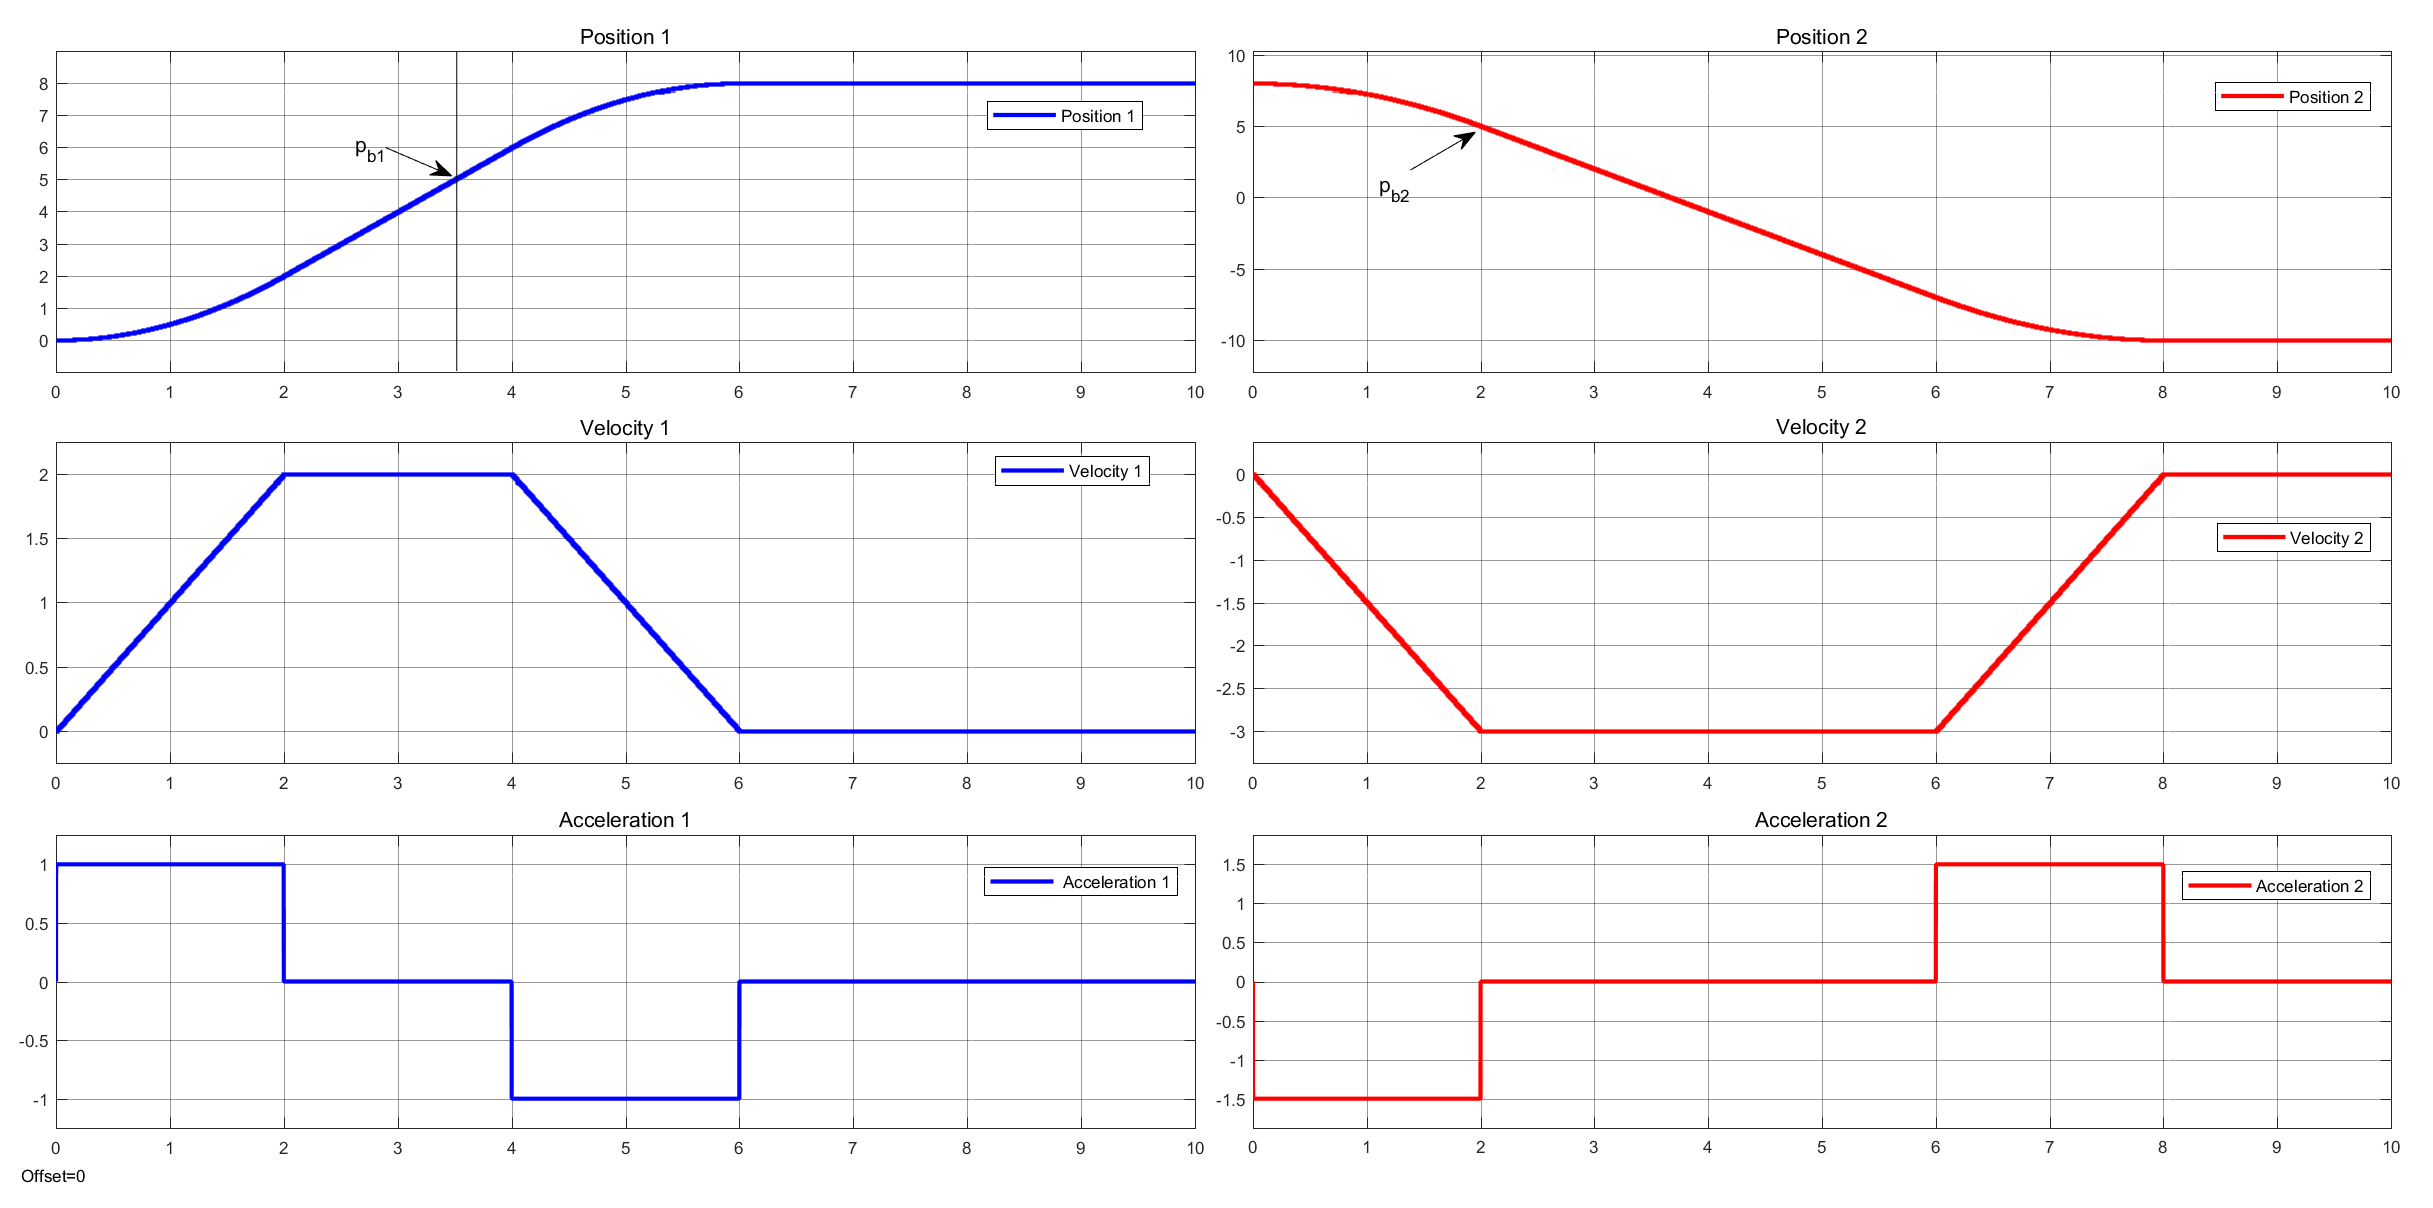
\includegraphics[width=0.9\columnwidth]{figure/original_trajectories.eps}%
	\caption{One-dimensional linear trajectory}%
	\label{ori_traj}
	\end{figure}

	\item According to the blending radius $r$, the points $p_{b1}$ on $x_1(t)$ and $p_{b2}$ on $x_2(t)$ which intersects with the blending sphere are computed. We also compute the durations $d_1$ for moving from $p_{b1}$ to $p_2$ on $x_1$ and $d_2$ for moving from $p_2$ to $p_{b2}$ on $x_2$. The transition window should start earliest from the time of $p_{b1}$ on $x_1(t)$ is reached, and ends latest at the time of $p_{b2}$ on $x_2(t)$ is reached. In the example, we take $r=3$ and $p_{b1} = p_{b2} = 5$ (see Figure.\ref{ori_traj}).

	\item Timely shift the $x_2(t)$ and select the transition window time $T$ according to the above rules. In order to avoid stop on the blending trajectory, the time shift $T_s$ of $x_2(t)$ should be smaller than the duration of $x_1(t)$. We now have the second trajectory as $x_2(t-T_s)$ for blending. In the example the duration of $x_1(t)$ is $6s$. Figure.\ref{blend_case_1} shows a blending case that we shift the $x_2(t)$ with $6s$, which is almost the same as motion without blending. Figure.\ref{blend_case_2} shows a blending case that we shift the $x_2(t)$ with $3.5s$ and the blending starts at 3.5s, ends at 5.5s. Figure.\ref{blend_case_3} shows a blending case that we shift the $x_2(t)$ with $4.5s$ and the blending starts at 3.5s, ends at 6.5s.
\end{enumerate}

In the actual implementation, we make the following choice given the durations $d_1$ and $d_2$ inside the blending sphere:
\begin{itemize}
\item If $d_1\leq d_2$ we shift exactly to the time when $p_{b1}$ is reached on $x_1$ (when the blending sphere is entered),
\item if $d_1>d_2$ we compute $T_s$ such that $T_s+d_2=T_1$. This choice minimizes increases in acceleration/deceleration on the resulting blend trajectory.
\end{itemize}


\section{Blending the orientation}
To blend the orientation, the method described in \cite{dantam2014orientation} is used. The equations (18)-(20) in \cite{dantam2014orientation} are used to calculate the orientation along the blend trajectory. In our application, due to the fact that the orientation change along the original (not blended) trajectories has smooth acceleration and deceleration phases, (18) and (19) from paper \cite{dantam2014orientation} do not need to be calculated.\newline
For the sake of clarity, it is important to note that our functions for $u_{ij}(t)$ and $u_{jk}(t)$ are different. However, we account for this difference by not explicitly calculating (18) and (19) and using the given samples of the original (not blended) trajectories instead. Furthermore,  (\ref{eq:2}) is used for $u_{j}(t)$, in other words, $u_{j}(t) = \alpha(s(t))$.


\begin{figure}[ht]
	\vspace*{-5mm}
	\centering
	\begin{subfigure}[ht]{0.8\textwidth}%
		\centering
		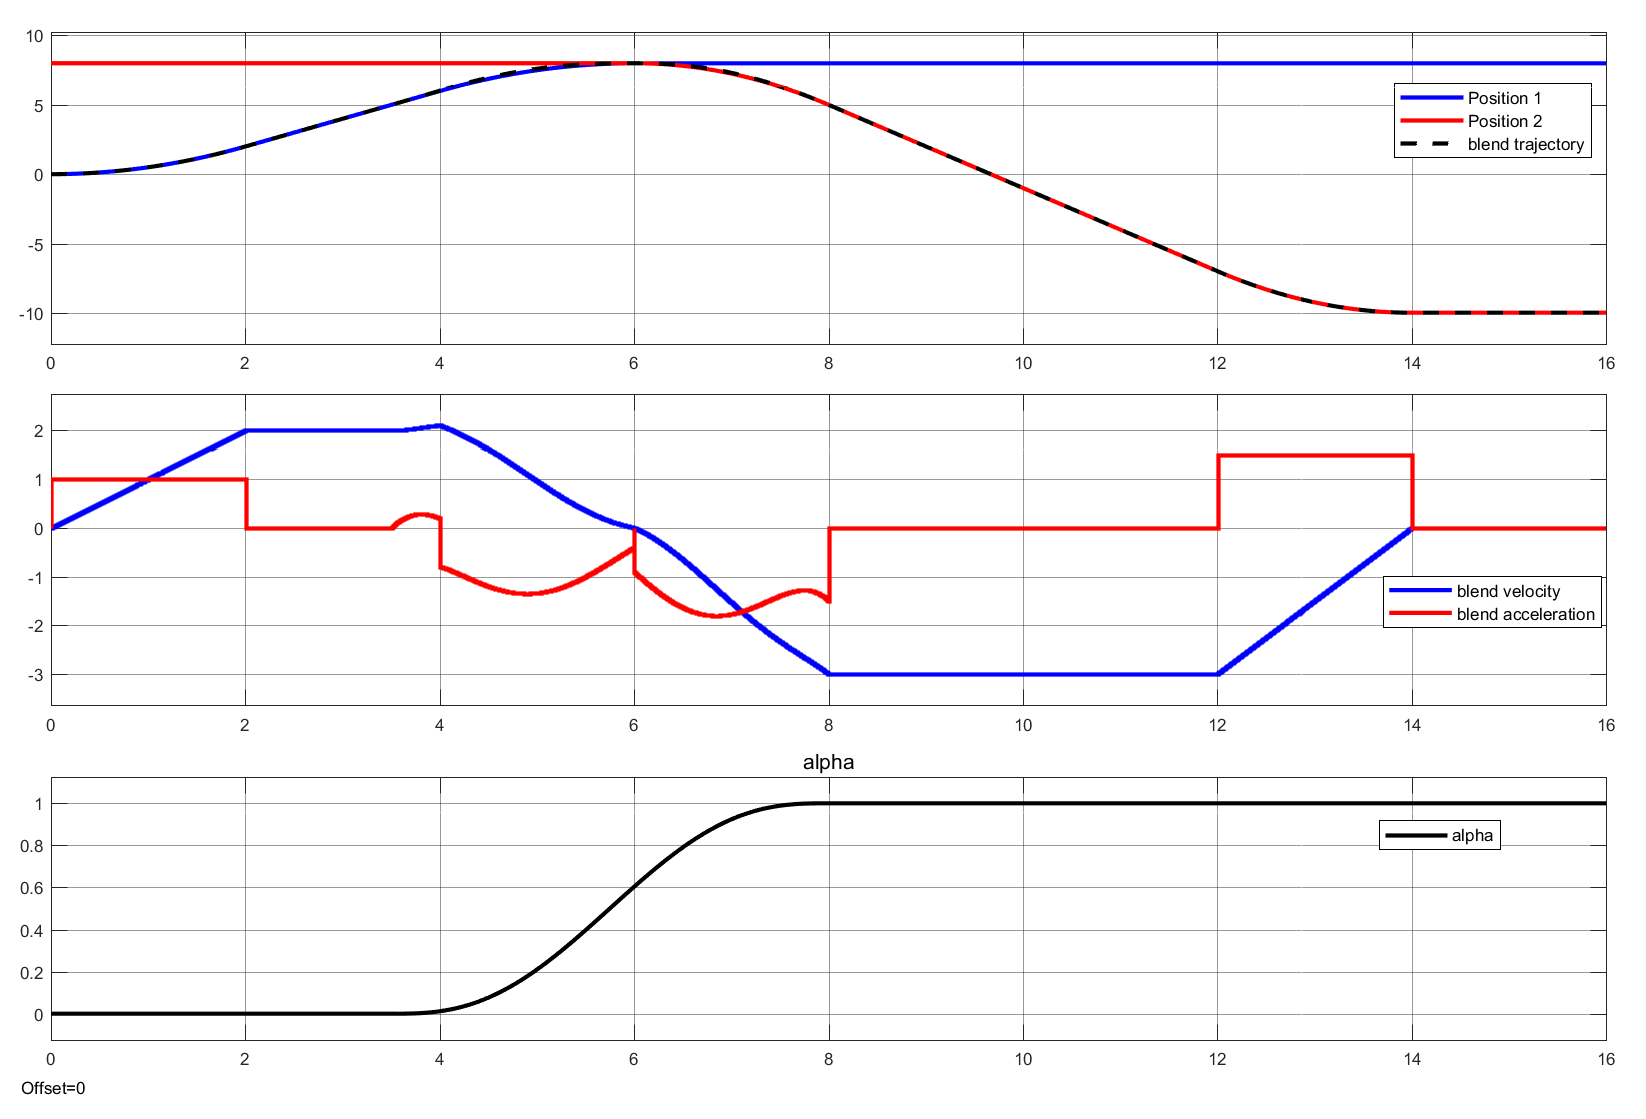
\includegraphics[width=0.8\columnwidth]{figure/blend_case_1.eps}%
		\caption{Motion blend case 1: $T_s = 6s$, blending starts at 3.5s, ends at 8s. The resulted blending trajectory comes to a stop in the middle.}%
		\label{blend_case_1}%
	\end{subfigure}
	
	\begin{subfigure}[ht]{0.8\textwidth}%
		\centering
		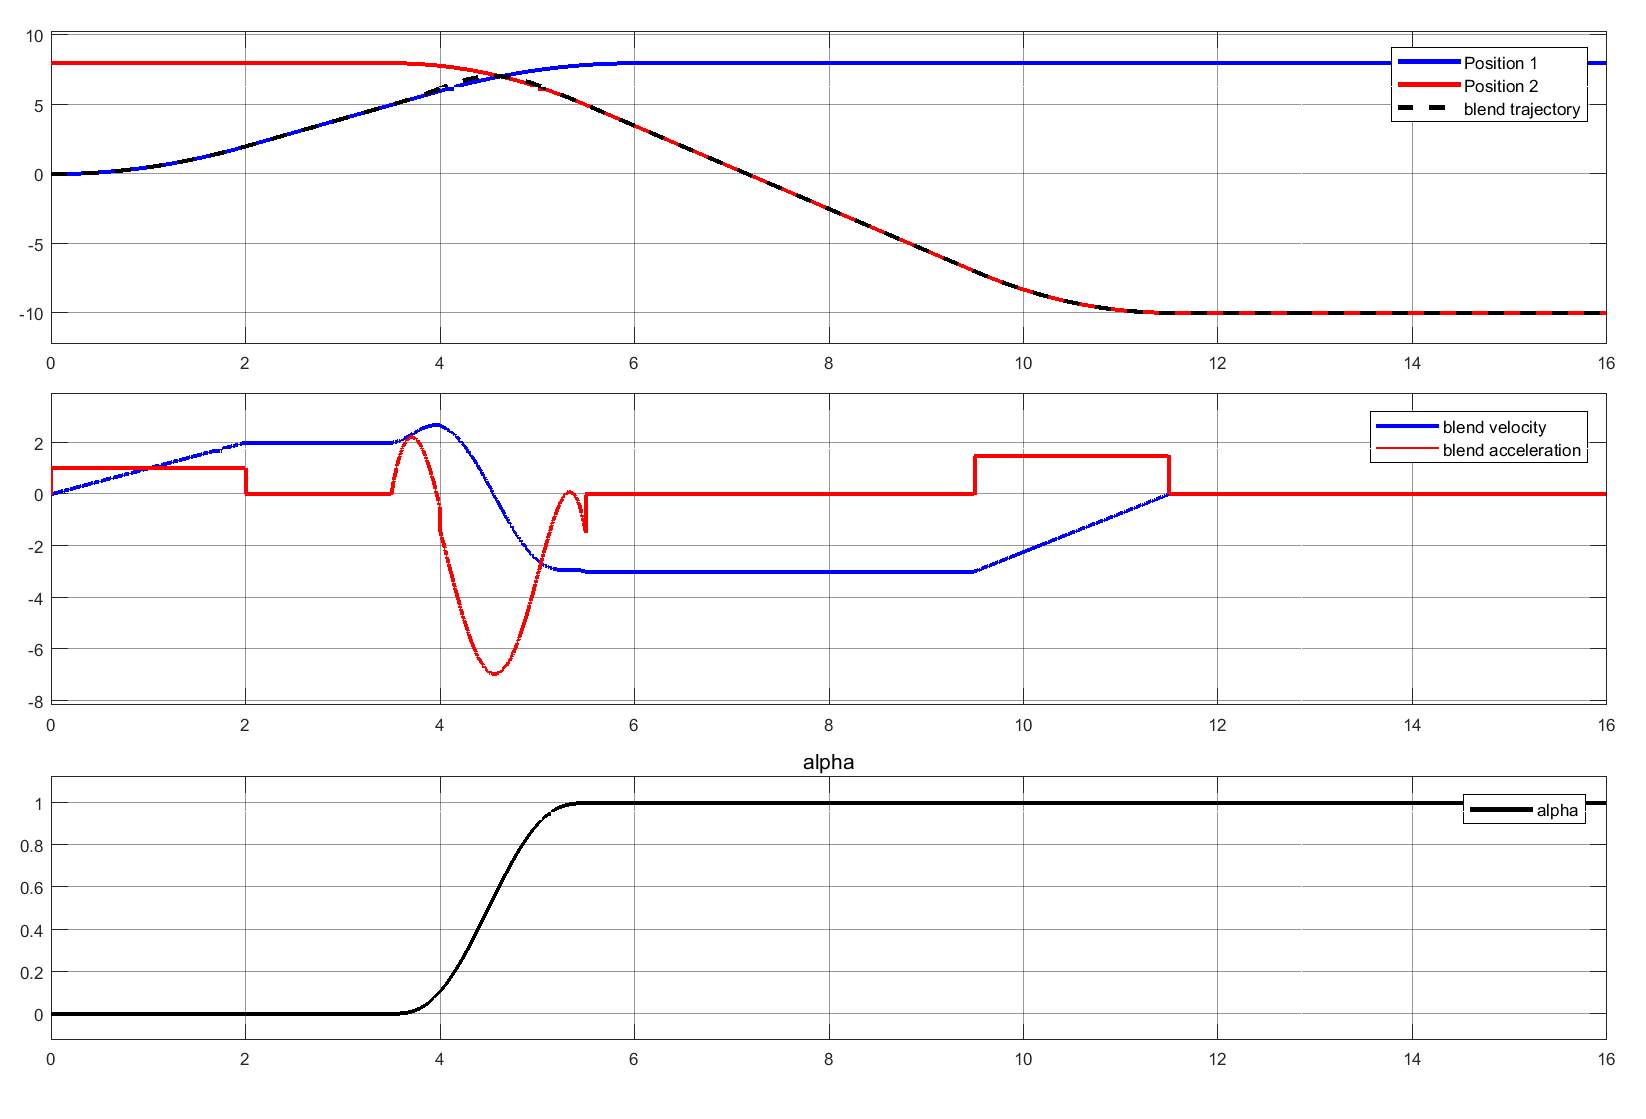
\includegraphics[width=0.8\columnwidth]{figure/blend_case_2.eps}%
		\caption{Motion blend case 2: $T_s = 3.5s$, blending starts at 3.5s, ends at 5.5s. The resulted blending trajectory smoothly transits from first trajectory to the second trajectory. The velocity profile has no jumps.}%
		\label{blend_case_2}%
	\end{subfigure}
	
	\begin{subfigure}[ht]{0.8\textwidth}%
		\centering
		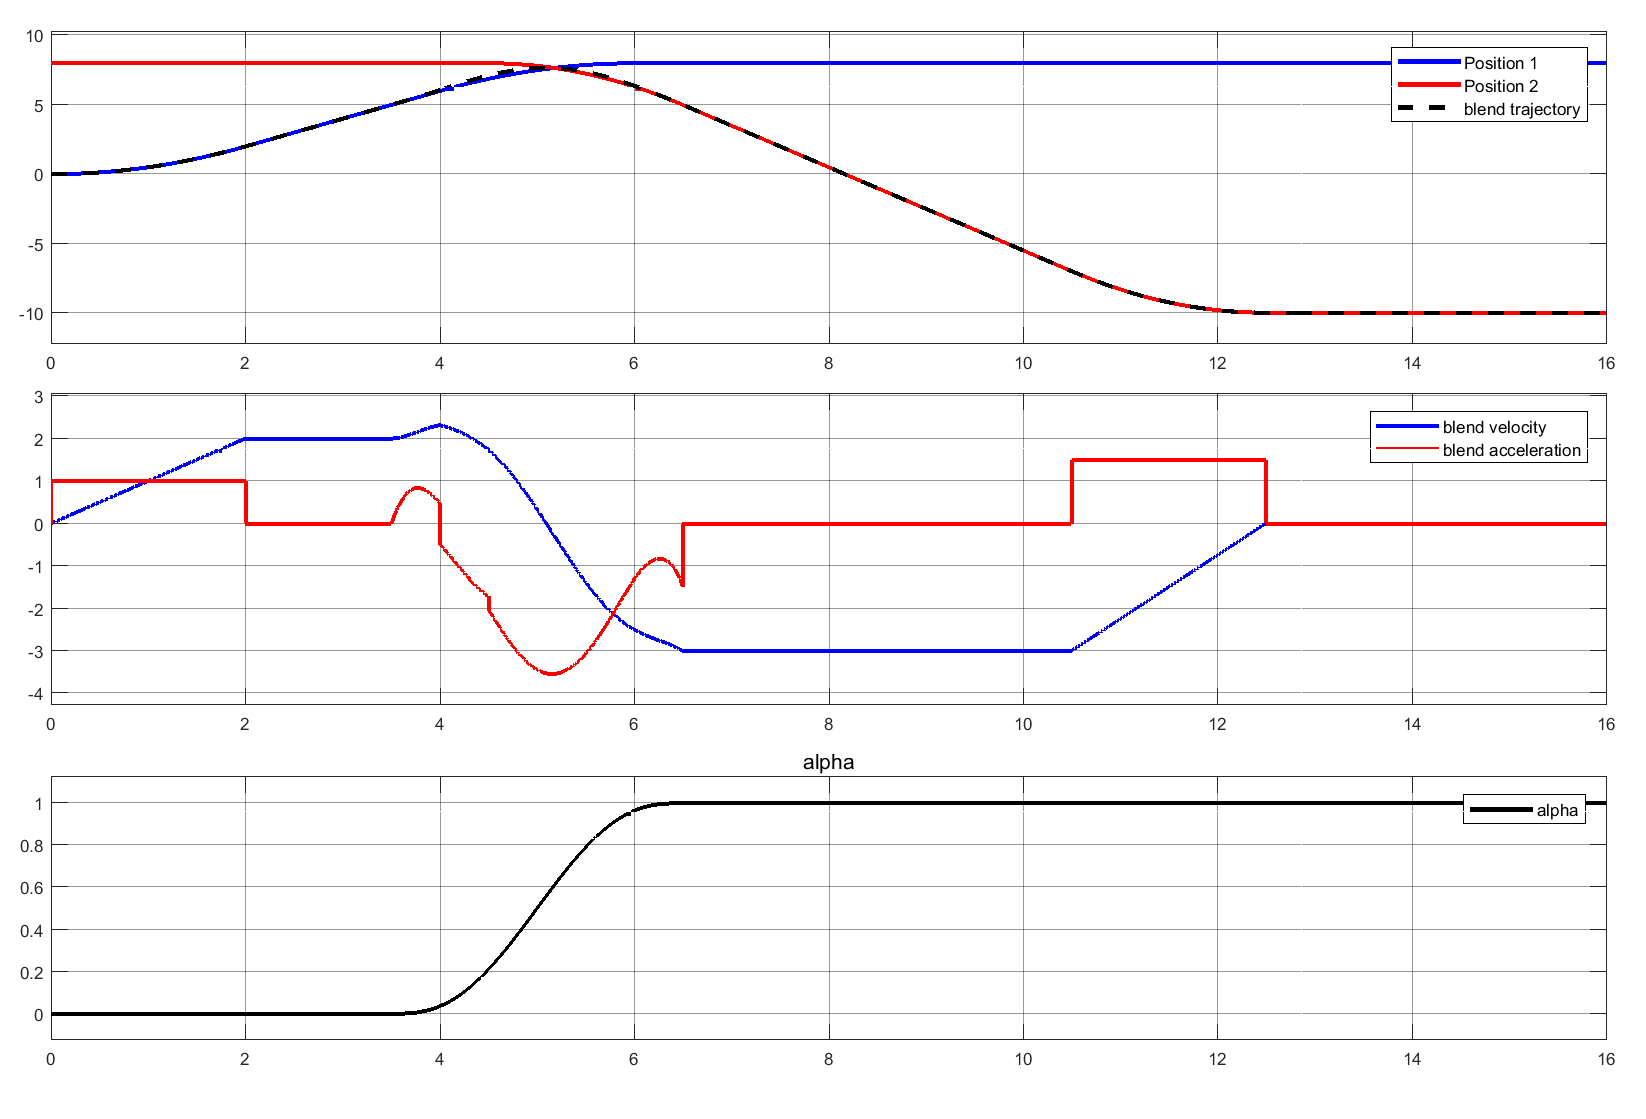
\includegraphics[width=0.8\columnwidth]{figure/blend_case_3.eps}%
		\caption{Motion blend case 3: $T_s = 4.5s$, blending starts at 3.5s, ends at 6.5s. The resulted blending trajectory smoothly transits from first trajectory to the second trajectory. The velocity profile has no jumps.}%
		\label{blend_case_3}%
	\end{subfigure}
	
\end{figure}


\begin{thebibliography}{9}
\bibitem {lloyd1993trajectory}Lloyd, John and Hayward, Vincent \textit{Trajectory generation for sensor-driven and time-varying tasks}, The International journal of robotics research, 1993
\bibitem {dantam2014orientation}Dantam, Neil and Stilman, Mike \textit{Spherical Parabolic Blends for Robot Workspace Trajectories}, International Conference on Intelligent Robots and Systems (IROS), 2014
\bibitem{pilztrajectorygeneration}\url{https://github.com/PilzDE/pilz_industrial_motion/tree/melodic-devel/pilz_trajectory_generation}
\end{thebibliography}
\end{document}
